\documentclass[12 pt]{article}
\hbadness=10
\usepackage[table]{xcolor}

\usepackage{amsmath, amssymb, amsfonts, setspace, stmaryrd, amsthm, graphicx, tikz,enumitem}

\usepackage[utf8]{inputenc}
\usepackage[english]{babel}
\usepackage{pgfplots}
\usetikzlibrary{positioning}% To get more advances positioning options
\usetikzlibrary{arrows}% To get more arrow heads


\usepackage[margin=1.5in]{geometry}



\newtheorem{theorem}{Theorem}
\newtheorem{remark}{Remark}
\newtheorem*{note}{Note}
%%align* environment
\newcommand{\eq}[1]{\begin{align*}#1\end{align*}}


%Math commands
\DeclareMathOperator{\R}{\mathbb{R}}
\DeclareMathOperator{\C}{\mathbb{C}}
\DeclareMathOperator{\Z}{\mathbb{Z}}
\DeclareMathOperator{\N}{\mathbb{N}}
\DeclareMathOperator{\Q}{\mathbb{Q}}
\DeclareMathOperator{\F}{\mathbb{F}}
\newcommand{\Mod}{\text{ mod }}
\newcommand{\cc}{\cellcolor}

\renewcommand\abstractname{Introduction}

\newcounter{exercise}[section]
\newenvironment{exercise}{\refstepcounter{exercise}\par\bigskip \begin{quotation}{}{\leftmargin .25in\rightmargin .25in}
	\noindent \textbf{Exercise~\thesection.\theexercise }  \rmfamily}{\end{quotation}\par\bigskip}
	

\newenvironment{bonus}{\refstepcounter{exercise}\par\bigskip \begin{quotation}{}{\leftmargin .25in\rightmargin .25in}
	\noindent \textbf{*Bonus Exercise*~\thesection.\theexercise }  \rmfamily}{\end{quotation}\par\bigskip}
	 


\title{Elliptic Curve Cryptography}
\author{Girls Talk Math}
\date{}

\begin{document}
\maketitle
\vskip 1in
\begin{center} \textbf{Introduction} \end{center}

Elliptic curve cryptography is an exciting application of the techniques of algebraic geometry and abstract algebra applied to the ancient art of keeping messages secure; furthermore, it is a hot topic and is on the verge of being implemented as a standard security protocol. Elliptic curves themselves are ubiquitous in mathematics. They arose historically in calculus but eventually made their way into geometry and algebra. Hopefully this document will serve as a smooth, practical introduction into the many beautiful areas of mathematics necessary to understand how elliptic curve cryptography works. We assume the reader knows only about complex numbers, basic algebra (equations for lines), and good old-fashioned long division. If things get confusing, discuss among your group and talk to your team leader.

\bigskip
If you see (*) this means the exercise is potentially very long or that the section is not strictly necessary for cryptography.
\smallskip
One last note about reading mathematical texts: It is very normal when reading math to read a passage or even a single sentence several times before you understand it properly. Also, never trust the author! Check every claim and calculation (time permitting). Take your time and never give up. Let's talk math!
\newpage

\tableofcontents

%%%%%%%%%%%%%%%%%%%%%%
%%% Use \section{}, \subsection{}, etc. for different parts of the problem set. Start a newpage for a new section
%%%%%%%%%%%%%%%%%%%%%%

%%%%%%%%%%%%%%%%%%%%%%%%%%%%%%%%%
%%%
%%% Embed exercises in section as appropriate 
%%% 
%%%%%%%%%%%%%%%%%%%%%%%%%%%%%%%%%%%

\newpage



\section{Modular Arithmetic}
\subsection{Introduction}
This section is foundational for everything to come (and is useful in many areas of mathematics and computer science).

Let's rephrase what you already know about division with remainder. For any integers $n,d$ there are unique integers $q,r$ such that $n=qd+r$ and $0 \leq r<d$. Here unique means that if $n=qd+r$ and $n=q'd+r'$ and both $r$ and $r'$ are in the range $[0,d)$, then it must be true that $q=q'$ and $r=r'$. You may have called $n$ the dividend, $d$ the divisor, $q$ the quotient, and $r$ the remainder. For example, $5=1*3+2$ and $29=2*13+3$; these expressions are concise summaries of the division procedure you may have learned earlier in life:

\begin{center}
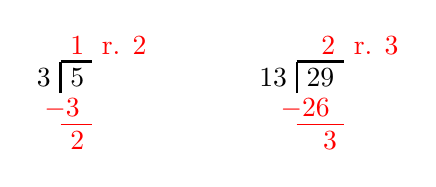
\begin{tikzpicture}
\draw[thick,-] (-1.5,-0.2) -- (-1.5,0.2);
\draw[thick,-] (-1.5,0.2) -- (-1.1,0.2);
\node[left] at (-1.5,0) {$3$};
\node[right] at (-1.5,0) {$5$};
\node[right,red] at (-1.5,0.4) {$1$};
\node[right,red] at (-1.83,-0.4) {$-3$};
\draw[red,-] (-1.5,-0.6) -- (-1.1,-0.6);
\node[right,red] at (-1.5,-0.8) {$2$};
\node[right,red] at (-1.1,0.4) {r. $2$};
%%%%%%%%%%%%%%%%%%%%%%%%%%%%%%%%%
\draw[thick,-] (1.5,-0.2) -- (1.5,0.2);
\draw[thick,-] (1.5,0.2) -- (2.1,0.2);
\node[left] at (1.5,0) {$13$};
\node[right] at (1.5,0) {$29$};
\node[right,red] at (1.69,0.4) {$2$};
\node[right,red] at (1.17,-0.4) {$-26$};
\draw[red,-] (1.5,-0.6) -- (2.1,-0.6);
\node[right,red] at (1.71,-0.8) {$3$};
\node[right,red] at (2.1,0.4) {r. $3$};
\end{tikzpicture}
\end{center}

On many occasions we only care about the remainder after division. For instance, consider an analog clock. If it reads 5 o'clock, what time will it read in 134 hours? Well, since the clock displays 12 hours in a circular manner we can solve this problem by simply dividing by 12: $5+134=11*12+7$. So the clock will read 7. This is an example of modular arithmetic in action.

Another example is the basic concepts of odd and even. A number is even if its remainder when divided by 2 is 0 and is considered odd if this remainder is 1.

\begin{exercise}
If an analog clock reads $8$ o'clock now, what time will it read in 112 hours?
\end{exercise}

\begin{exercise}
If the minute hand on an analog clock reads $55$ now, what minute will it read in $413$ minutes?
\end{exercise}

\subsection{Modular Notation}
We will change notation later to emphasize a different aspect, but the following notation is standard in all of mathematics. Let $a,b$ be integers and $n$ be a nonzero integer. We write $a\equiv b\text{ mod }n$ (and we read ``$a$ is congruent to $b$ modulo $n$'') if $a$ and $b$ have the same remainder when dividing by $n$. For example, $25\equiv 9\mod 4$. In particular, note that if $r$ is the remainder of $a$ divided by $n$, $a\equiv r \Mod n$. 

\begin{exercise}
Find the remainder of 120 divided by 12 and express this in modular notation. Do the same for 39 divided by 5.
\end{exercise}

\subsection{Finiteness}
Notice that when we divide an integer by $n$ the remainder is always an integer between 0 and $n-1$. Therefore every number is congruent modulo $n$ to a number between 0 and $n-1$. This finiteness is one reason modular arithmetic is so useful: to check a property for all integers modulo $n$ we only need to check it for the integers 0 to $n-1$.

\subsection{Arithmetic}
Let's look at some examples of how remainders behave upon addition and multiplication. Note that $29=2*13+3$ and $100=7*13+9$ which means $29\equiv 3\Mod 13$ and $100\equiv 9\Mod 13$. Observe that
\[
100+29=129=9*13+12,
\]
and that $12=3+9$. Thus in our notation $100+29\equiv 9+3 \Mod 13$. This example illustrates a general truth: addition is preserved by taking remainders. The same is true for multiplication:
\[
100*29=2900=223*13+1.
\]
This means $100*29\equiv 1\Mod 13$ and $9*3=27=2*13+1$ so we have that $9*3\equiv 1\Mod 13$. Therefore $100*29\equiv 9*3 \Mod 13$, and again this is an illustration of a general truth: multiplication is also preserved by taking remainders.

Since our usual operations on numbers are preserved by taking remainders, and since there are only finitely many such remainders, this motivates the following new structure (a set of symbols with additional properties) which we call ``the integers modulo $n$.'' We denote this new structure by $\Z_n$.

Fix a positive integer $n$. Consider the set of symbols $[0],[1],...,[n-1]$.  This set is what we call $\Z_n$. We define operations on these symbols via taking remainders:

\begin{center}
\begin{enumerate}
\item $[k]+[l]=[$\text{remainder of }$k+l$\text{ when divided by }$n]$
\item $[k]*[l]=[$\text{remainder of }$k*l$\text{ when divided by }$n]$
\end{enumerate}
\end{center}
where $k$ and $l$ belong to $0,1,...,n-1$.

For example, if $n=13$ then $\Z_{13}=\{[0],[1],[2],[3],[4],[5],[6],[7],[8],[9],$\linebreak$[10],[11],[12]\}$ with rules 1 and 2 above. Some sample calculations (check these!) are
\[
[10]*[11]=[6]
\]
and $[12]+[12]=[11]$.

\begin{exercise}
Write out $\Z_5$ and $\Z_8$. In $\Z_5$ compute $[4]+[4]$. In $\Z_{13}$ compute $[5]*[11]$ and $[9]+[8]$.
\end{exercise}

Often times we will abuse notation and write a number larger than $n-1$ in brackets then reduce it modulo $n$. For example, in $\Z_5$ we may write 

\[[3]+[3]=[6]=[1]\] 
because  $6\equiv 1\Mod 5$. Also, we use the notation $k[l]$ to indicate the sum of $[l]$ with itself $k$ times. We use the notation $-[l]$ to indicate the unique element of $\Z_n$ which satisfies $-[l]+[l]=[0]$. Note that $[-k]=-[k]$ because 
\[[-k]+[k]=[\text{remainder of }k-k\Mod n]=[0]. \]
Here are some examples of computing ``negatives'' in $\Z_{13}$.
\begin{align*}
-[5]&=[-5]=[8] \\
-[6]&=[-6]=[7] \\
-[3]&=[-3]=[10]
\end{align*}
since $-5\equiv 8\mod 13$ for the first. You should check the second and third examples.

\begin{remark}
Some people like to imagine $\Z_n$ as a ``number circle'' since \[[n-1]+[1]=[0].\] Therefore adding $[1]$ to itself repeatedly cycles through all elements of $\Z_n$. Compare this to the discussion about clocks at the beginning of section 1. Calculating what time a clock will say later is merely a calculation in $\Z_{12}$!
\end{remark}

\begin{exercise}
Compute $[-3]$ in $\Z_5$ and $\Z_6$. Also compute \\$[12]+[-5]*[2]$ in $\Z_{13}$.
\end{exercise}

\subsection{$\Z_p$ when $p$ is prime}
Recall that a natural number $p$ is prime if its only factors are $1$ and $p$ (by convention, $1$ is not prime). The first few primes are $2$, $3$, $5$, $7$, and $11$. 

When we consider $\Z_p$ when $p$ is prime, $\Z_p$ has a property that makes it even closer to behaving like regular numbers. This is the following:
\begin{center}
For every element $[n]\not =[0]$ in $\Z_p$, there is another element $[m]$ such that $[n]*[m]=[1]$. We call $[m]$ the \textit{multiplicative inverse} of $[n]$.
\end{center}
For example, we have already seen that $[9]*[3]=[1]$ in $\Z_{13}$, so $[3]$ is the multiplicative inverse of $[9]$ (in $\Z_{13}$). The above property (every non-zero element has a multiplicative inverse) is satisfied by the rational, real and complex numbers. For example, the inverse of $1+i$ in the complex numbers is $\frac{1}{2}-\frac{1}{2}i$ because 
\[
(1+i)*\left(\frac{1}{2}-\frac{1}{2}i\right)=1.
\]

Let us discuss some notation related to multiplicative inverses. It is traditional to denote the multiplicative inverse by using $-1$ as an exponent e.g. $[9]^{-1}=[3]$ in $\Z_{13}$. Later, when we write $\frac{a}{b}$ we actually mean $a*b^{-1}$. For example, in $\Z_{13}$ we have 

\[\frac{[2]}{[9]}=[2]*[9]^{-1}=[2]*[3]=[6].\]

\begin{exercise}
Compute $[3]^{-1}$ and $\frac{[1]}{[2]}$ in $\Z_5$ and $\Z_7$.
\end{exercise}

\begin{exercise}
In $\Z_4$, calculate $[2]*[2]$. Does $[2]$ have a multiplicative inverse? Notice that 4 is not prime.
\end{exercise}

\newpage
\section{Group Theory}
\subsection{Introduction - Symmetries of an Equilateral Triangle}
The origins of group theory lie in the study of symmetries. A motivating example is the set of symmetries of an equilateral triangle.

\begin{center}
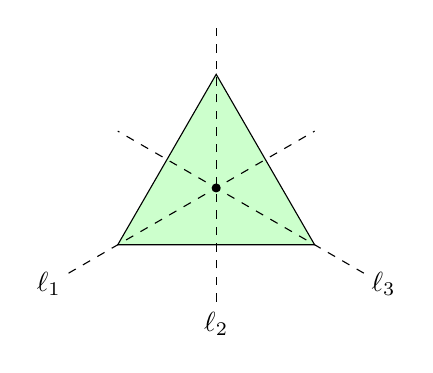
\begin{tikzpicture}[scale=2.5]
\filldraw[fill=green!20] (-0.5,0) -- (0.5,0) -- (0,0.86603) -- cycle;
\draw[dashed] (0,-.28867) -- (0,1.1);
\draw[dashed] (0.75,-0.14434) -- (-0.5,0.57735);
\draw[dashed] (-0.75,-0.14434) -- (0.5,0.57735);

\node at (-0.85,-0.2) {$\ell_1$};
\node at (0,-.4) {$\ell_2$};
\node at (0.85,-0.2) {$\ell_3$};

\draw[fill = black, radius=0.02] (0,0.28868) circle;
\end{tikzpicture}
\end{center}

A ``symmetry'' of this equilateral triangle is a rigid motion (reflection, rotation, translation) that places the triangle back on top of itself. For instance, reflecting (or flipping) the triangle across the line labeled $\ell_1$ is such a rigid motion; let's call this rigid motion $F_1$. Similarly, let $F_2$ and $F_3$ stand for the reflections across lines $\ell_2$ and $\ell_3$. Rotating the triangle about the center point by $120$ degrees counter-clockwise is also a symmetry; let's call this rigid motion $R_{120}$. There are two other rotation symmetries: one which rotates by $0$ degrees and one by $240$ degrees counter-clockwise about that same point (call these $R_0$ and $R_{240}$ for consistency). 

The crucial observation is this: two symmetries of the equilateral can be ``put together'' in a meaningful way. If, say, one flips the triangle over $\ell_1$ and then rotates it counter-clockwise by $120$ degrees, what is the resulting rigid motion?  Let's label the corners of the triangle to make it clear:

\begin{center}
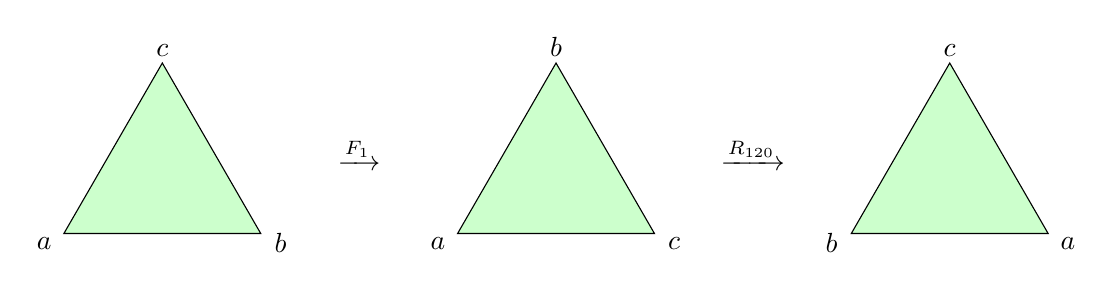
\begin{tikzpicture}[scale=2.5]
\filldraw[fill=green!20] (-2.5,0) -- (-1.5,0) -- (-2,0.86603) -- cycle;
\node at (-2.6,-0.05) {$a$};
\node at (-1.4,-0.05) {$b$};
\node at (-2,0.93) {$c$};

\node at (-1,0.4) {$\xrightarrow{F_1}$};

\filldraw[fill=green!20] (-0.5,0) -- (0.5,0) -- (0,0.86603) -- cycle;
\node at (-0.6,-0.05) {$a$};
\node at (0.6,-0.05) {$c$};
\node at (0,0.95) {$b$};

\node at (1,0.4) {$\xrightarrow{R_{120}}$};

\filldraw[fill=green!20] (1.5,0) -- (2.5,0) -- (2,0.86603) -- cycle;
\node at (1.4,-0.05) {$b$};
\node at (2.6,-0.05) {$a$};
\node at (2,0.93) {$c$};

\end{tikzpicture}
\end{center}

The end result is that the triangle has been flipped across $\ell_2$ (notice how the corners labelled $a$ and $b$ switched places, but the corner labelled $c$ stayed put). The two rigid motions $F_1$ and $R_{120}$ were ``composed'' to yield a different rigid motion: $F_2$. Let's write this as $F_1* R_{120}=F_2$. 

\begin{exercise}
Explain why $R_{120}*R_{120}=R_{240}$.
\end{exercise}

\begin{exercise}
Explain why $R_{120}*R_{240}=R_0$.
\end{exercise}

\begin{exercise}
What is $F_1*F_2$? Is it the same as $F_2*F_1$?
\end{exercise}


\subsection{Group - Formal Definition}
A group, often denoted $G$, is a set of elements that obey a few rules:
\begin{enumerate}[label=(\roman*)]
\item If $a$ and $b$ are elements of $G$, then we can ``multiply'' them to get a third element $c$ of $G$; we write this as $a*b=c$. (It does not need to be true that $a*b=b*a$.) This property is commonly called ``closure.'' The $*$ is called the ``operation'' of the group. 
\item There is one special element of $G$ called the ``identity'' which we shall usually call $e$; it has the unique property that $e*a=a*e=a$ for any element $a$.
\item If $a$ is an element of $G$, then there is a unique element $b$ called the ``inverse'' of $a$; it satisfies the property $a*b=b*a=e$. Sometimes we write this inverse element as $a^{-1}$. Note that $e^{-1}=e$.
\item If $a,b,c$ are three elements of $G$, then $a*(b*c)=(a*b)*c$; that is, the operation is ``associative.''
\end{enumerate}
At first glance, that looks like a long and tedious list of rules. Actually, you're probably quite familiar with a few groups already:

\begin{enumerate}[label=$\bullet$]
\item The integers, commonly denoted $\mathbb{Z}$, is the group $\{\hdots,-2,-1,0,1,2,\hdots\}$ where the operation is regular addition. Instead of $*$, we usually use the $+$ symbol; e.g., $5+8=13$. The identity element is $0$ since $z+0=z=0+z$ for any integer $z$. The inverse of $17$ is $-17$, etc. The group of integers has an additional special property: if $a$ and $b$ are any integers then $a+b=b+a$. A group that possesses this property is called ``Abelian'' after the mathematician Niels Abel. With the same operation, the rational numbers (denoted $\mathbb{Q}$), the real numbers (denoted $\mathbb{R}$), and the complex numbers (denoted $\mathbb{C}$) are also Abelian groups. 
\item The rational numbers except for $0$ (we write $\mathbb{Q}\setminus \{0\}$) form a group whose operation is regular multiplication. That is, $\frac{a}{b}\cdot\frac{c}{d} = \frac{ac}{bd}$, for any non-zero integers $a,b,c,d$. The identity of this group is $1$, and the inverse of $\frac{a}{b}$ is $\frac{b}{a}$. This group is also Abelian. 
\item The set of symmetries of an equilateral triangle form a group whose operation is what we referred to above as composition (e.g., $F_1*R_{120}=F_2$). This group has a standard name: $D_3$. It is the simplest example of a group which is not Abelian. 
\end{enumerate}


Here's an example that builds on the modular arithmetic from the previous section. First, consider $\Z_4$. This forms a group under modular addition (e.g., $[3]+[2]=[1]$, $[2]+[1]=[3]$). Let's summarize the operation for this group with a table (commonly called a Cayley Table):
\begin{center}
\begin{tabular}{|c||c|c|c|c|}
\hline
+ & \cc{blue!15}0 & \cc{green!15}1 & \cc{yellow!15}2 & \cc{red!15}3 \\ \hline\hline
\cc{blue!15}0 & \cc{blue!15}0 & \cc{green!15}1 & \cc{yellow!15}2 & \cc{red!15}3 \\\hline
\cc{green!15}1 & \cc{green!15}1 & \cc{yellow!15}2 & \cc{red!15}3 & \cc{blue!15}0 \\\hline
\cc{yellow!15}2 & \cc{yellow!15}2 & \cc{red!15}3 & \cc{blue!15}0 & \cc{green!15}1 \\\hline
\cc{red!15}3 & \cc{red!15}3 & \cc{blue!15}0 & \cc{green!15}1 & \cc{yellow!15}2 \\\hline
\end{tabular}
\end{center}
From the coloring of entries, we can observe that (apart from the top and side labels) each element in $\Z_4$ appears exactly once in each row and column. This is a visualization of the ``inverse'' and ``closure'' properties above. In addition, we observe that the $[0]$ row and the $[0]$ column are copies of the top labels and side labels, respectively. This is a visualization of the ``identity'' property (the identity of this group is $[0]$). The ``associative'' property is not obvious from this table. Finally, we observe that, because the table has symmetry across the lower-right diagonal, the group is Abelian.  Can you explain this connection? 

\begin{exercise}
Summarize the operation of the group of symmetries of an equilateral triangle (i.e. $D_3$) in a Cayley table. Fill in each entry with the resulting motion when the motion on the left is performed first, followed by the motion on the top. You may split up the work among your group members. 
\begin{center}
\begin{tabular}{|c||c|c|c|c|c|c|}
\hline
$*$ & ~~~$R_0$~~~ & ~~~$R_{120}$~~~ & ~~~$R_{240}$~~~ & ~~~$F_1$~~~ & ~~~$F_2$~~~ & ~~~$F_3$~~~ \\\hline
& & & & & & \\
$R_0$ & & & & & & \\
& & & & & & \\\hline
& & & & & & \\
$R_{120}$ & & $R_{240}$ & $R_{0}$ & & & \\
& & & & & & \\\hline
& & & & & & \\
$R_{240}$ & & & & & & \\
& & & & & & \\\hline
& & & & & & \\
$F_1$ & & $F_2$ & & & & \\
& & & & & & \\\hline
& & & & & & \\
$F_2$ & & & & & & \\
& & & & & & \\\hline
& & & & & & \\
$F_3$ & & & & & & \\
& & & & & & \\\hline
\end{tabular}
\end{center}
\end{exercise}

\begin{remark}
Rule (ii) in the definition of a group says there must be only one special element called the identity. Actually, this rule could require only that there is \emph{an} identity element, without specifying that there is only one. That is, if $e$ and $f$ are elements of $G$, both of which behave like identity elements, then $e=f$ must be true. This is because $e*f=e$ (since $f$ is an identity) and $e*f=f$ (since $e$ is an identity), and therefore $e=e*f=f$. 
\end{remark}

\subsection{Isomorphic Groups}

Now consider $\Z_5$. If we exclude $[0]$ from this set, the resulting set (we write $\Z_5\setminus\{[0]\}$) is a group under modular multiplication (e.g., $[3]\cdot [2]=[1], [2]\cdot [2]=[4]$). Let's also visualize this group operation in a Cayley Table:

\begin{center}
\begin{tabular}{|c||c|c|c|c|}
\hline
$\cdot$ & \cc{blue!15}1 & \cc{green!15}2 & \cc{yellow!15}4 & \cc{red!15}3 \\\hline\hline 
\cc{blue!15}1 & \cc{blue!15}1 & \cc{green!15}2 & \cc{yellow!15}4 & \cc{red!15}3 \\\hline
\cc{green!15}2 & \cc{green!15}2 & \cc{yellow!15}4 & \cc{red!15}3 & \cc{blue!15}1 \\\hline
\cc{yellow!15}4 & \cc{yellow!15}4 & \cc{red!15}3 & \cc{blue!15}1 & \cc{green!15}2 \\\hline
\cc{red!15}3 & \cc{red!15}3 & \cc{blue!15}1 & \cc{green!15}2 & \cc{yellow!15}4 \\\hline
\end{tabular}
\end{center}
Do you notice anything in common about the colors in this Cayley table and the Cayley table for $\Z_4$? The elements of both groups have been ordered and given colors in such a way that the colored Cayley Tables are identical. The elements of the groups themselves are not the same ($[0]$ is the identity of the first, and $[1]$ is the identity of the second), but they are, in some sense, the ``same'' group. More precisely, the groups are the same if we re-label the elements. Even more precisely, we can set up a one-to-one correspondence between the elements of $\Z_4$ and $\Z_5\backslash \{[0]\}$ as follows: 
\begin{align*}
[0]&\leftrightarrow [1]\\
[1]&\leftrightarrow [2]\\
[2] & \leftrightarrow [4]\\
[3] & \leftrightarrow [3]
\end{align*}
This correspondence is exactly the one alluded to by the coloring, and it {\it respects} the different operations of the two groups: for example, the statement $[2]+[3] = [1]$, which is true for the group on the left, corresponds to the statement $[4]\cdot [3] = [2]$ on the right exactly by replacing $[2]$ with $[4]$, $[3]$ with $[3]$, $[1]$ with $[2]$, \emph{and} the ``$+$'' symbol with the ``$\cdot$'' symbol. When two groups have such a correspondence, we call them ``isomorphic'' groups. 

The correspondence between $\Z_4$ and $\Z_5\setminus\{[0]\}$ just described may seem non-obvious. Why are the elements of $\Z_5\setminus\{[0]\}$ ordered $[1],[2],[4],[3]$, while those of $\Z_4$ maintain the order $[0],[1],[2],[3]$? To understand this better, we need the notion of generators; Section 3.5 will have more to say about this example. 

\begin{exercise}
Explain why every group is isomorphic to itself. That is, what is the correspondence? 
\end{exercise}

\begin{exercise}
Explain why $\Z_3$ and $\Z_4$ are not isomorphic. (Hint: how many elements are in each group?)
\end{exercise}

\begin{exercise}
The groups $\Z_6$ and $D_3$ both have $6$ elements. Decide whether or not they are isomorphic. (Hint: are they both Abelian?)
\end{exercise}

\subsection{Generators}
In an arbitrary group, there may be many elements and/or a complicated group operation. It is often helpful in such cases to identify certain elements of the group from which the rest of the group derives its structure. Let's begin with a few examples. 

Recall from above that the set of integers, $\Z$, is a group with the operation of regular addition. There are infinitely many elements in $\Z$, but they are all derived from a single special element: $1$. For instance, $5$ is nothing except the addition of $1$ with itself $5$ times: $1+1+1+1+1=5$. There is nothing special about $5$; any natural number $n$ can be written as the sum of $1$s: 
$$
n=\underbrace{1+1+\hdots+1}_{n\text{ of these}}
$$
Furthermore, $0$ can be thought of as an empty sum of $1$s, and any negative number can be written as the sum of $-1$s. So every element of $\Z$ is either the identity element, a sum of $1$s, or a sum of $-1$s. This motivates the following definition: 

A collection $S$ of (some or all of the) elements of a group $G$  (we write $S\subset G$ for ease of notation) is a \emph{generating set} for $G$ if every element of $G$ is 
\begin{enumerate}[label=(\roman*)]
\item the identity of $G$, or
\item equal to a product $a_1*a_2*\cdots *a_n$ where each $a_j$ is either an element of $S$ or the inverse of an element of $S$ (here ``$*$'' denotes the group operation, not necessarily regular multiplication).
\end{enumerate}
The elements of $S$ are, in this case, called \emph{generators} of $G$. Of course, any group can be generated by the set $S=G$; however, the most interesting generating sets are those with only a few elements. 

In the example above, $\{1\}$ is a generating set for $\Z$; indeed all of $\Z$ can be generated by the single element $1$. Note that $\{-1\}$ is also a generating set for $\Z$, since in general the elements of the generating set, along with their inverses, can be used to comprise all other elements of the group. Finally, $\{2\}$ is not a generating set for $\Z$; sums of $2$s or $-2$s are always even integers, so no odd integer can be written as a sum of $2$s or $-2$s. 

Groups that can be generated by a single element (like $\Z$, for example) are called \emph{cyclic}. For such a group, it is often interesting to discuss which of its elements can, by themselves, generate the whole group. 

\begin{exercise}
Explain why $\{4,5\}$ is a generating set for $\Z$. (Hint: can you write $1$ as a sum of $\pm 4$s and $\pm 5$s?)
\end{exercise}

\begin{bonus}
Explain why the following is true: if $G$ is a cyclic group, then $G$ is Abelian. (Hint: fix a generator $a$ for the group. Let $x,y$ be arbitrary elements of $G$, and assume you can write $x=a^m=\underbrace{a*a*\cdots*a}_{m\text{ of these}}$ and $y=a^n=\underbrace{a*a*\cdots*a}_{n\text{ of these}}$. Show that $x*y=y*x$. Then generalize your argument to account for when $x$ or $y$ is a product of $a^{-1}$s instead of $a$s.)
\end{bonus}

For a second example, consider again the modular arithmetic group $\Z_4$. Here the element $[1]$ is a generator since the non-zero elements of $\Z_4$ can be expressed as sums of $[1]$s: 
$$
[1] = [1]; \quad [2] = [1]+[1]; \quad [3] = [1]+[1]+[1]
$$
So $\Z_4$ is a cyclic group. Another element which serves as a generator for $\Z_4$ is $[3]$:
$$
[1]=[3]+[3]+[3]; \quad [2]=[3]+[3]; \quad [3]=[3]
$$
But $[2]$ is not a generator for the group since $[2]+[2]=[0]$ and therefore any sum of $[2]$s is either equal to $[0]$ or $[2]$, never $[1]$ or $[3]$. 

Actually, this example extends more generally: every group $\Z_{n}$ is cyclic and generated by $[1]$. Remember that earlier remark about imagining $\Z_n$ as a ``number circle?'' It's no mistake that our ``number circles'' are cyclic. 

\begin{exercise}
If $p$ is a prime number, explain why $\Z_p$ can be generated by every non-zero element. Review Section 2.5 if necessary, and use the fact that $[m]\cdot[n]=m[n]$ in any $\Z_n$. 
\end{exercise}

For a third and last example, recall the group $D_3$ of symmetries of an equilateral triangle. For this group, $\{R_{120},F_1\}$ is a generating set. For example, $R_{240}=R_{120}*R_{120}$ and $F_2=F_1*R_{120}$. 

\begin{exercise}
Write $F_3$ as a product of $R_{120}$s and $F_1$s, completing the explanation that every non-identity element of $D_3$ can be written as such. 
\end{exercise}

\begin{remark}
The group $D_3$ can't be generated by a single element because then it would be cyclic, which would make it Abelian (see the starred exercise above). Therefore the generating set $\{R_{120},F_1\}$ is as small as any generating set could possibly be for $D_3$. 
\end{remark}

\begin{remark}
There do, however, exist Abelian groups that aren't cyclic. See the next exercise for an example, if you're interested.
\end{remark}

\begin{bonus}
The set of symmetries of a non-square rectangle is 
$$
\{R_0,R_{180},F_1,F_2\},
$$
where $R_n$ means rotation by $n$ degrees counterclockwise, and $F_1$ and $F_2$ are the lateral and longitudinal flips (it doesn't matter which is which). This set forms a group with the same operation as $D_3$; it is called $D_2$. 
\begin{enumerate}[label=\arabic*.]
\item Show that for any element $a$ in this group, $a*a$ is the identity $R_0$. Explain why this means the group can't be generated by a single element. 
\item Write down a Cayley table for this group to show that the group is Abelian (i.e., observe that the Cayley table has diagonal symmetry). 
\end{enumerate}
\end{bonus}

\subsection{Generators and Isomorphic Groups}

To conclude our discussion of generators of groups, let's revisit the concept of isomorphic groups. If a group $G$ is isomorphic to a group $H$, then a few things must already be true: if $G$ and $H$ are finite, they must each have the same number of elements; $G$ is Abelian if $H$ is and vice-versa; the one-to-one correspondence between $G$ and $H$ must pair the two identity elements together. Now we're ready to add another item to the list. 

If $G$ and $H$ are isomorphic groups, the correspondence between them must also induce a correspondence between generating sets. That is, if $S\subset G$ is a generating set for $G$, then the elements of $H$ corresponding to $S$ (call them $S'$, say) form a generating set for $H$. This property is true simply because the correspondence between $G$ and $H$ must respect the operation in both groups (you may wish to think about this more carefully on your own.) 

The main application of this discussion is this: if two cyclic groups are isomorphic, then the correspondence between them must pair generators together. Actually, even more is true: if $G$ and $H$ are cyclic groups of the same size, then they are automatically isomorphic via any one-to-one correspondence that sends a generator of $G$ to a generator of $H$ and respects the operations. 

As an example: the correspondence between $\Z_4$ and $\Z_5\setminus\{[0]\}$ in Section 3.3 paired $[1]$ (from $\Z_4$) with $[2]$ (from the second group). Indeed, $[2]$ is a generator for $\Z_5\setminus\{[0]\}$ since the non-identity elements can be expressed as products of $[2]$s:
$$
[2]=[2]; \quad [2]\cdot[2]\cdot[2]=[3]; \quad [2]\cdot[2]=[4]
$$

Another correspondence could have been chosen: since the multiplicative inverse of $[2]$ (which is $[3]$) is an equally good generator for $\Z_5\setminus\{[0]\}$, we could have instead paired $[1]\leftrightarrow [3]$ and so on. 

\begin{exercise}
Set up a correspondence between the elements of $\Z_6$ and the elements of $\Z_7\setminus\{[0]\}$ that respects the operations of the two groups, thereby showing that the two groups are isomorphic. Do this by finding a generator, $a$, for the second group and pairing $[1]\leftrightarrow a$, $[2]\leftrightarrow a\cdot a$, etc. 
\end{exercise}


%\begin{remark}
%One of the most beautiful and impressive results in the area of group theory is the collection of theorems called Sylow's Theorems. An easy and elegant consequence of Sylow's Theorems is the following true statement: if $p$ is a prime number, then $(p-1)! = (p-1)\times (p-2)\times \cdots \times 2\times 1$ is congruent to $p-1 \mod p$. So indeed, the humble beginnings of modular arithmetic help inform our understanding of groups, which in turn help us understand modular arithmetic. 
%\end{remark}

\newpage
\section{Finite Fields}

\subsection{Introduction}
In the last section you learned about groups -- algebraic structures with a single well-behaved operation. In this section we will discuss another algebraic structure, which we call a ``field'', that possesses two well-behaved operations which resemble addition and multiplication

As with groups, you are already familiar with some examples of fields. For instance, the rational ($\Q$), real ($\R$), and complex ($\C$) numbers with the usual addition and multiplication are fields. Note that the usual multiplication has the following properties:
\begin{enumerate}[label=(\roman*)]
\item Multiplication is associative: $a*(b*c)=(a*b)*c$.
\item There is an identity, namely 1: $1*z=z*1$ for any non-zero number $z$. 
\item For any nonzero number $z$ there is an inverse $z^{-1}$ such that $zz^{-1}=z^{-1}z=1$.
\item The multiplication is commutative (if you want to be fancy you can summarize the properties up to here by saying that the nonzero elements of a field form an abelian group with respect to multiplication).
\item The distributive property holds: $z(a+b)=za+zb$. You can think of this property as a rule that makes the multiplication and addition compatible.
\end{enumerate}
As stated in the group theory section, $\Q,\R$, and $\C$ are abelian groups with respect to addition -- this combined with the above rules for multiplication are what makes these sets of numbers \emph{fields}.


\subsection{$\Z_p$ as a field}
In the modular arithmetic section you secretly learned about another field: the remainders modulo a prime number $p$ (Recall we denoted this set $\Z_p$). To be precise, multiplication of remainders modulo $p$ is an associative, commutative operation with an identity element ($[1]$), and it is possible to divide by any nonzero remainder. Furthermore, multiplication distributes over addition modulo $p$ just as it does in the usual sense. The fields $\Z_p$ are called \emph{finite fields} simply because they are also finite sets. This gives a lot of examples of finite fields -- one for each prime $p$ (there are infinitely many primes); it turns out there are more finite fields than just $\Z_p$.

When we wish to emphasize that we are viewing $\Z_p$ as a field and not just as an abelian group it is customary to use the notation $\F_p$.

\begin{exercise}
Here is some more practice doing modular calculations. Calculate $[5]/[9]$ in $\F_{13}$ and $\F_{17}$. Recall the notation from section 2.5.
\end{exercise}

\subsection{Extensions of $\F_p$ ($*$)}
Let us begin this subsection with a helpful comparison to the relationship between the real numbers $\R$ and the complex numbers $\C$. Every element of $\C$ is written $a+bi$ where $a$ and $b$ are real numbers and $i$ is a solution to $x^2+1=0$. It is important here that the polynomial $x^2+1$ does not factor into the product of two pieces which have coefficients in $\R$, otherwise all roots of $x^2+1$ would belong to $\R$ and there would be nothing special about $i$.

To paraphrase the last paragraph, the complex numbers are an extension of the real numbers where we have added a root of the irreducible (this means it doesn't factor) polynomial $x^2+1$. An amazing fact is that we can use the same procedure to create extensions of $\F_p$. Let's look at some examples:

Consider the finite field $\F_3$. Note that the multiplicative inverse of $[2]$ is $[2]$ itself. Therefore $[0]^2=[0]$, $[1]^2=[1]$ and $[2]^2=[1]$ which means that $[2]$ is not the square of any element of $\F_3$. That is, $[2]$ does not have a square root in $\F_3$. We may create an extension of $\F_3$, which we will denote $\F_{3^2}$ or $\F_9$, by adding the square root of $[2]$ to $\F_3$. Explicitly, the elements of $\F_{3^2}$ are of the form $a+b\theta$ where $a$ and $b$ are in $\F_3$ and $\theta^2=[2]$ (or if you wish $\theta$ is a solution of $x^2+[1]=0$ because $[2]=[-1]$). The following is a sample calculation in $\F_{3^2}$. Note how similar it is to calculating in the complex numbers:

\begin{align*}
([2]+[1]\theta)*([1]+[2]\theta)&=[2]*[1]+[1]*[1]\theta+[2]*[2]\theta+[1]*[2]\theta^2 \\
&=[2]+[2]\theta+[2]\theta^2 \\
&=[2]+[2]\theta+[2]*[2] \\
&=[2]+[2]\theta+[1] \\
&=[2]\theta
\end{align*}
From now on instead of writing $[1]\theta$, we will just write $\theta$.

\begin{exercise}
How many elements are there in $\F_{3^2}$? (Use the explicit form of the elements $a+b\theta$).
\end{exercise}

\begin{exercise}
Compute $([2]+[2]\theta)^2$ and $([1]+[1]\theta)^3$ in $\F_{3^2}$ where $\theta^2=[2]$.
\end{exercise}

\begin{exercise}
Find $([2]+[2]\theta)^{-1}$ in $\F_{3^2}$ (Try to use the same method you would for complex numbers).
\end{exercise}

Now we will consider an extension of $\F_3$ that is slightly different from our analogy with $\R$ and $\C$ . We create this extension, called $\F_{3^3}$ by adding a solution of $x^3+x^2+[2]=0$. Explicitly, the elements of $\F_{3^3}$ are of the form $a+b\theta+c\theta^2$ where $a,b$ and $c$ are in $\F_3$ and $\theta^3=-\theta^2-[2]$. Here is a sample calculation in $\F_{3^3}$:

\begin{align*}
([1]+\theta+\theta^2)^2&=[1]+[2]\theta+[3]\theta^2+[2]\theta^3+\theta^4 \\
&=[1]+[2]\theta+[3]\theta^2+\theta^3([2]+\theta) \\
&=[1]+[2]\theta+[3]\theta^2+(-\theta^2-[2])([2]+\theta) \\
&=[1]+[2]\theta+[3]\theta^2-[2]\theta^2-[4]-\theta^3-[2]\theta \\
&=\theta^2-\theta^3 \\
&=\theta^2-(-\theta^2-[2]) \\
&=[2]+[2]\theta^2
\end{align*}
On the third and sixth steps we have used that $\theta^3=-\theta^2-[2]$. Also since $[3]=[0]$ we have could have eliminated $[3]\theta^2$ on the first step.

The previous extension of $\F_3$ may be a little surprising since the standard form for an element has three terms $(a+b\theta+c\theta^2)$ instead of two like in the complex numbers (actually there is no equivalent of the last example for $\R$). In general, there may be an arbitrary number of terms but from now on we will only use examples which have two terms $(a+b\theta)$ to simplify examples.

\begin{remark}
In general, you can not use an arbitrary polynomial to make a field extension -- it needs to be irreducible. Also, the number of terms in the standard form of an element in a field extension is often called the \emph{degree} of the field extension. The degree of $\F_{3^2}$ is 2 and the degree of $\F_{3^3}$ is 3.
\end{remark}

\begin{exercise}
Compute $(1+[2]\theta)(\theta+\theta^2)$ in $\F_{3^3}$ where $\theta^3+\theta^2+[2]=[0]$.
\end{exercise}

\begin{exercise}
We want to emphasize that for $n>1$, $\F_{p^n}\not=\Z_{p^n}$ even though $\Z_p=\F_{p}$. Does the element $[3]$ in $\Z_{3^2}$ have a multiplicative inverse (if you forgot what this means see section 2.5)? Compare this with the fact that every nonzero element of $\F_{3^2}$ has an inverse.
\end{exercise}

\begin{bonus}
In $\F_5$ the perfect squares are $[0]$,$[1]$ and $[4]$. Therefore we can create two extensions: the first by adding a square root of $[2]$ and the second by adding a square root of $[3]$. It turns out these extensions actually have the same ``structure''. If you have time (this will take awhile), your group should try to compare the Cayley tables for multiplication for both extensions and observe that they are ``isomorphic'' as groups. Review section 2 if necessary!
\end{bonus}

\subsection{Characteristic of a Finite Field}
There is a major difference between doing arithmetic in a finite field versus the usual number systems $\Q, \R$ and $\C$. For a finite field, there is a smallest number $p$, which we call the \emph{characteristic} of the field, such that any element added to itself $p$ times equals zero: $p*t=0$ for any $t$ in the finite field $\F$. Compare this to the situation for ordinary numbers where no matter how many times you add 1 to itself the result will never be equal to 0. We write $\text{Char}(\F)$ to denote the characteristic of $\F$.

\begin{exercise}
What is the characteristic of $\F_2$? $\F_3$? What about $\F_{3^2}$ as defined above? $\F_p$? 
\end{exercise}

When we study elliptic curves later we will only use finite fields which do not have characteristic equal to 2 or 3. This restriction simplifies the exposition because in characteristic 2 or 3 the definition of an elliptic curve is more complicated.
 
\newpage
\section{Projective Geometry ($*$)}
This section is optional. If you are running short on time feel free to skip it. The motivation for this section is that elliptic curves have a ``point at infinity'' and we make this notion precise using projective geometry. If you do skip this section just view the point at infinity as an element ``infinitely far away'' from the other points on the curve.

\subsection{Introduction}
The origins of projective geometry date back to at least the Renaissance. Artists sought to create realistic perspectives and to do so became interested in the apparent ``points at infinity'' that occur on the horizon. You are probably familiar with the picture below of two parallel lines that appear to ``intersect at infinity''.

\begin{center}
\begin{tikzpicture}
%\draw[help lines] (0,0) grid (3,3);
\draw (-1,3) -- (4,3);
\draw (.5,0) -- (1.5,3);
\draw (2.5,0) -- (1.5,3);

\node [above] at (1.5,3) {$\infty$};
\end{tikzpicture}
\end{center}

\subsection{The Projective Line}
Before we discuss how to construct a plane with points at infinity (which is the case we will need for elliptic curves) we will show you how to make precise the notion of a line with a point at infinity. This is easier and gets the main idea across.
\newpage
Consider the picture below:
\begin{center}
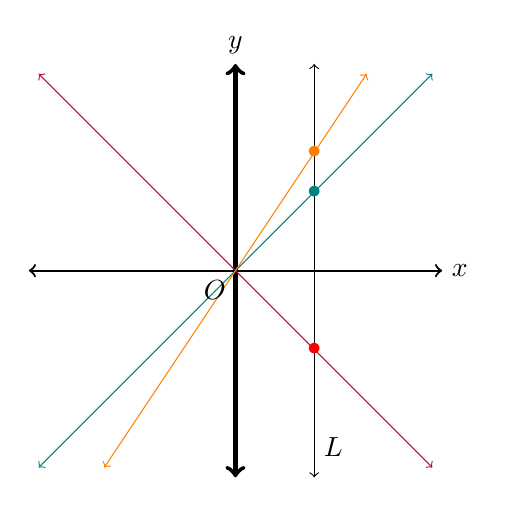
\begin{tikzpicture}[scale=.5]
%\draw[help lines] (-5,-5) grid (5,5);
\draw [ultra thick, <->] (0,-5.25) -- (0,5.25);
\draw [thick, <->] (-5.25,0) -- (5.25,0);
\draw [<->] (2,-5.25) -- (2,5.25);
\draw [purple, <->] (-5,5) -- (5,-5);
\draw [teal, <->] (5,5) -- (-5,-5);
\draw [orange, <->] (-10/3,-5) -- (10/3,5);


\node [below right] at (2,-4) {$L$};
\node [above] at (0,5.25) {$y$};
\node [right] at (5.25,0) {$x$};
\node [orange] at (2,3) {$\bullet$};
\node [teal] at (2,2) {$\bullet$};
\node [red] at (2,-2) {$\bullet$};
\node [below left] at (0,0) {$O$};

\end{tikzpicture}
\end{center}

Notice that every line through the origin $O$ except the $y$-axis intersects $L$ once. Also note that as a point crawls up $L$, the slope of the corresponding line through $O$ is getting steeper and steeper. Since we generally think of the $y$-axis as having infinite slope, this is a good candidate for our ``point at infinity''.

\begin{exercise}
Let $L$ be the line in the plane defined by the equation $x=1$. For the points $(1,5)$, $(1,10)$ and $(1,100)$ on $L$, calculate the slope of the corresponding line that intersects $O=(0,0)$. Notice that the slopes are increasing.
\end{exercise}

To make the above description precise algebraically we need a good notation for writing lines through $O$. The standard notation for this is called \emph{homogeneous coordinates}. We describe these coordinates now. Consider ordered pairs $[x:y]$ where $x,y$ are real numbers, not both equal to zero. We let $[x:y]$ be equal to $[c*x:c*y]$ for any nonzero number $c$ and write $[x:y]=[c*x:c*y]$. The reason we force all nonzero scalar multiples of $[x:y]$ to be equal is because $(x,y)$ and $(c*x,c*y)$ are on the same line with slope $(cy)/(cx)=y/x$ in the usual plane; thus $[x:y]$ represents a line through the origin.

\begin{exercise}
Which lines through $O$ do the homogeneous coordinates $[3:4]$, $[10:14]$, $[0:1]$ and $[1:0]$ represent?
\end{exercise}

If $x\not=0$, we may divide both coordinates in $[x:y]$ by $x$, so we have $[1:y/x]=[x:y]$. Letting $z=y/x$ we have $[1:z]$ where $z$ is \emph{any} number. Points of this form, $[1:z]$, correspond to points on $L$ in our picture! But there is one extra point which occurs when $x=0$, $[0:1]$, the point at infinity. We call the collection of all homogeneous coordinates $[x:y]$ subject to the rules described in the paragraph before exercise 4.2 the \emph{projective line}.

\subsection{The Projective Plane}
The projective plane is defined very similarly to the projective line and again we use homogeneous coordinates. We take ordered triples $[x:y:z]$ where not all coordinates are zero and we say that $[x:y:z]=[c*x:c*y:c*z]$ for all nonzero numbers $c$. This time points of the form $[1:y:z]$ form the usual points in the plane and points of the form $[0:y:z]$ form the ``projective line at infinity'' (there is a whole line at infinity now!). The point $[0:0:1]$ may be thought of as ``the point at infinity of the line at infinity'' (relax if this feels strange at first, it does to everyone).

Let's discuss how to calculate for a line in the usual plane its points at infinity. A line in the plane has an equation in standard form: $ay+bz=c$ where $y,z$ are variables and $a,b,c$ are constants. To find its points at infinity first we \emph{homogenize} it: $ay+bz=cx$. Then we substitute $x=0$ and see which points of the form $[0:y:z]$ satisfy the equation $ay+bz=0$. Here's an example:

For $3y+4z=2$, first we homogenize to obtain $3y+4z=2x$. Then we see that if $x=0$ that $y=\frac{-4}{3}z$. Therefore $[0:\frac{-4}{3}z:z]=[0:\frac{-4}{3}:1]$ is the point at infinity on $3y+4z=2$. We divided by $z$ since it cannot be zero; otherwise all coordinates would equal zero which is prohibited.

\begin{exercise}
Find the points at infinity on the lines $2y+12z=4$ and $y+z=0$.
\end{exercise}

\begin{exercise}
This exercise is about parallel lines intersecting at infinity like in the introduction of this section. Calculate the intersection of the parallel lines $y-3z=0$ and $y-3z=-1$ in homogeneous coordinates. To do this, calculate their points at infinity.
\end{exercise}

\subsection{Elliptic Curves}
Elliptic curves are curves in the plane defined by the equation 
\[
y^2=x^3+ax+b
\]
where $a$, $b$ are numbers which satisfy $-16(4a^3+27b^2)\not=0$. 

In the previous section when we homogenized an equation we added a third variable $x$. Here, since we are already using $x$; instead, we will use $z$.

To homogenize the above equation (and any equation) identify the term of highest degree, in our case $x^3$, and multiply the other terms by a power of $z$ which makes the ``total degree'' equal to the highest degree. For the above example we get:
\[
y^2z=x^3+axz^2+bz^3.
\]
To find the point at infinity we plug in $z=0$ to get
\[
0=x^3.
\]
This means that we must have $x=0$. So the point at infinity is $[0:y:0]=[0:1:0]$ where we have divided by $y$ again since it is not allowed to be equal to zero.

In what follows we will use the symbol $\infty$ to denote the point at infinity because we will not use homogeneous coordinates. Also, we will use finite fields instead of $\R$. If you want to challenge yourself after you are finished learning everything you may try proving $1$ and $2$ of the group law in section 6.1. For this you will need to use homogeneous coordinates.

\newpage
\section{Elliptic Curves over Finite Fields}
Elliptic curves (not just over finite fields) occur in many fields of mathematics and are quite important to our understanding of mathematics as a whole (especially number theory). In this section we introduce elliptic curves over finite fields and learn how to compute the set of points on the curve.

\subsection{Definition of Elliptic Curves}

An elliptic curve over a finite field $\F$ ($\text{Char}(\F)\not= 2, 3$), denoted $E_{\F}$ or just $E$, is the set of all points $(x,y)$ (and a point at infinity we call $\infty$) such that $x$, $y$ are in $\F$ and they satisfy
\[
y^2=x^3+ax+b
\]
where $a$ and $b$ are constants in $\F$ such that $-16(4a^3+27b^2)\not= [0]$. The value $\Delta=-16(4a^3+27b^2)$ is called the \emph{discriminant} of $E$. $\Delta$ is the greek letter capital ``Delta''. 

\begin{remark}
This remark concerns notation. If you did \emph{not} read the extensions of finite field section, whenever you see $E(\F)$ just read this as $E$. If you did read about finite fields continue. Suppose $K$ is an extension of $\F$ (e.g. remember $K=\F_{3^2}$ is an extension of $\F_3$). Then we can look for solutions of $y^2=x^3+ax+b$ (where $a,b$ are in $\F$) in the bigger field $K$. We let $E(K)$ denote the set of all solutions $(x,y)$ of the previous equation such that $x$ and $y$ are in $K$.
\end{remark}

\subsection{An Example}

We begin with an example of an elliptic curve over $\mathbb{F}_{13}$.
Let $E$ be the elliptic curve defined by the equation
\begin{align}
y^2=x^3+[3]x+[8]
\end{align}

To find the points of $E(\F_{13})$ we use the following algorithm:
\begin{enumerate}
\item Calculate all perfect squares over $\F_{13}$ (To do this square every element of $\F_{13}$).
\item For each element of $\F_{13}$, calculate $x^3+[3]x+[8]$ and determine if it is a perfect square. Throw away those elements of $\F_{13}$ such that $x^3+[3]x+8$ is not a perfect square.
\item Match the $x$-values calculated in step 2 with the corresponding $y$-values calculated in step 1 so that $(x,y)$ satisfies equation $(1)$.
\end{enumerate}

Below we present these steps worked out for $E(\F_{13})$,
\begin{enumerate}
\item \[\text{\begin{tabular}{c|c}
$y$ & $y^2$ \\ \hline
${[}0]^2$ & [0]  \\
${[}1]^2$ & [1]  \\
${[}2]^2$ & [4]  \\
${[}3]^2$ & [9]  \\
${[}4]^2$ & [3]  \\
${[}5]^2$ & [12]  \\
${[}6]^2$ & [10] \\
${[}7]^2$ & [10] \\
${[}8]^2$ & [12]  \\
${[}9]^2$ & [3]  \\
${[}10]^2$ & [9]  \\
${[}11]^2$ & [4]  \\
${[}12]^2$ & [1]  \\
\end{tabular}}\]
So the squares modulo 13 are $[0],[1],[3],[4],[9],[10],[12]$.
Notice the symmetry: we only need to check up to $(p-1)/2$ since $r^2\equiv (p-r)^2 \mod p$ (a fact you should check). \\
\hspace{1mm}
\item \[\text{\begin{tabular}{c|c}
$x$ & $x^3+[3]x+[8]$ \\ \hline
{[}0] & [8] \\
{[}1] & [12] \\
{[}2] & [9] \\
{[}3] & [5] \\
{[}4] & [6] \\
{[}5] & [5] \\
{[}6] & [8] \\
{[}7] & [8] \\
{[}8] & [11] \\
{[}9] & [10] \\
{[}10] & [11] \\
{[}11] & [7] \\
{[}12] & [4] 
\end{tabular}}\]

Thus the only elements of $\F_{13}$ that can possibly occur as $x$-coordinates of a point on $E$ are $x=[1],[2],[9],[12]$.

\item Hence the points on $E$ are $([1],[5])$, $([1],[8])$, $([2],[3])$,  $([2],[10])$, $([9],[6])$, $([9],[7])$, $([12],[2])$, $([12],[11])$ and $\infty$ (we always include $\infty$).

\begin{exercise}
Use the steps above to compute the points of the elliptic curve over $\F_5$ defined by the equation $y^2=x^3+[1]$. (In other words compute $E(\F_5)$.)
\end{exercise}

\begin{exercise}
Use the steps above to compute the points of the elliptic curve over $\F_5$
defined by the equation $y^2=x^3+x$. (In other words compute $E(\F_5)$.)
\end{exercise}

\begin{bonus}
For the same curve defined in the last exercise, compute $E(\F_{5^2})$. Construct $\F_{5^2}$ by adjoining a square root of 2 (This means the elements of $\F_{5^2}$ are of the form $x+y\theta$ where $\theta^2=2$ and where $x,y$ are in $\F_5$. (Note: This calculation is very long! Split this up among the group or just do as much as you can in a reasonable amount of time then check with the team leader.)
\end{bonus}

\end{enumerate}

\newpage
\section{Group law for Elliptic Curves}
\subsection{The Group Law}
Amazingly, elliptic curves are also groups. In this section we will learn the group operation for elliptic curves. As we shall see, this is essential for cryptographic applications of the subject.

The group operation is defined geometrically. Let $P=(a_1,b_1)$ and $Q=(a_2,b_2)$ be two points on an elliptic curve $E$. Consider the line $L$ that is defined by $P$ and $Q$
\[
L: y-b_1=\frac{b_2-b_1}{a_2-a_1}(x-a_1)
\]
where we used the point-slope formula. The \emph{sum} $R=(a_3,b_3)$, of $P$ and $Q$, is defined as follows: $L$ intersects $E$ in a third point. $R$ is the reflection of this third point across the $x$-axis. We usually just write $P+Q$ instead of $R$. See the figure below for a visualization.

\begin{note}
We define a \emph{reflection across the $x$-axis} by simply making the $y$-coordinate negative, that is send $(x,y)$ to $(x,-y)$. 
\end{note}

\begin{center}
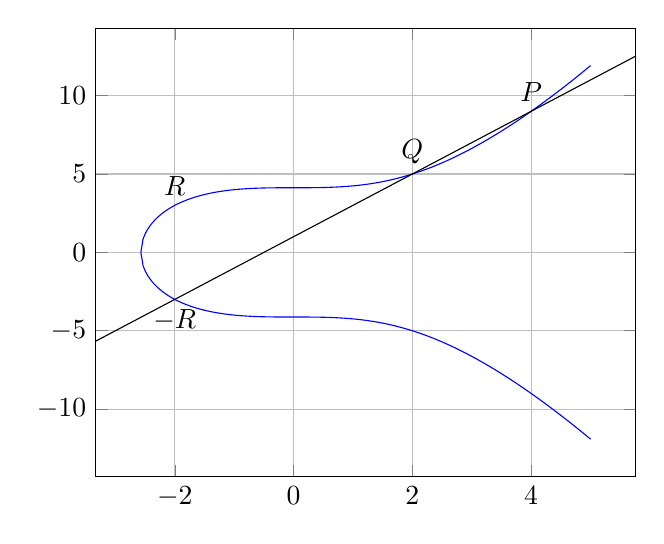
\begin{tikzpicture}
\begin{axis}[no marks,samples=200,domain=-2.571281:5,grid=both]
\addplot[blue] {sqrt(x^3+17)};
\addplot[blue] {-sqrt(x^3+17)};
\coordinate[label={90:$R$}] (R) at (axis cs:-2,3);
\coordinate[label={-90:$-R$}] (-R) at (axis cs:-2,-3);
\coordinate[label={90:$P$}] (P) at (axis cs:4,9);
\coordinate[label={90:$Q$}] (Q) at (axis cs:2,5);
\coordinate (a) at (axis cs:6,13);
\coordinate (b) at (axis cs:-4,-7);
\draw (a) -- (P) -- (Q) -- (-R) --(b) ;
\end{axis}
\end{tikzpicture}
\end{center}

The following theorem explicitly states the group law and the few exercises afterward will guide you through the proof of parts 3 and 4:

\begin{theorem}
Let $E$ be an elliptic curve defined over a finite field $\F$ (of $\operatorname{char}(\F)\not =2,3$) by the equation $y^2=x^3+ax+b$. Then the following hold:
\begin{enumerate}
\item \emph{Identity}. $P+\infty=\infty+P=P$ for all points $P$ on $E$. ($\infty$ is the identity of the group)
\item \emph{Negatives}. If $P=(x,y)$ is a point on $E$, then $(x,y)+(x,-y)=\infty$. The point$(x,-y)$ is denoted by $-P$ and is called the negative of $P$; note that $-P$ is a point on $E$. Also, $-\infty=\infty$.
\item \emph{Point addition}. Let $P=(a_1,b_1)$ be a point on $E$ and $Q=(a_2,b_2)$ be another point on $E$ such that $Q\not = \pm P$. Then $P+Q=(a_3,b_3)$, where
\begin{align*}
a_3=\left(\frac{b_2-b_1}{a_2-a_1}\right)^2-a_1-a_2, && b_3=\left(\frac{b_2-b_1}{a_2-a_1}\right)(a_1-a_3)-b_1
\end{align*}
\item \emph{Point doubling}.If $P=(a_1,b_1)$ is a point on $E$, where $P\not =-P$. Then $2P=(a_3,b_3)$, where
\begin{align*}
a_3=\left(\frac{3a_1^2+a}{2b_1}\right)^2-2a_1, && b_3=\left(\frac{3a_1^2+a}{2b_1}\right)(a_1-a_3)-b_1.
\end{align*}
\end{enumerate}
\end{theorem}

\begin{remark}
You may wonder how you will ever get infinity when you add two finite points. If the denominators are 0 in the above formulas, then you arrived at $\infty$! Also part 1 above indicates that $\infty$ is the identity of the group. 
\end{remark}

The following observation will be useful in the next exercises: Expand the polynomial $(x-c_1)(x-c_2)(x-c_3)$ and note the formula for the coefficient of $x^2$. This will be useful when you need to find the third root of a cubic polynomial given that you know 2 solutions already.

\begin{exercise}\emph{Proof of point addition} \\ 
Let $P,Q$ be points on $E$ such that $Q\not=\pm P$. Use the line $L$ defined previously and the equation defining $E$ ($y^2=x^3+ax+b$) to solve for the coordinates of the third point $P+Q=(a_3,b_3)$ on $L$ and $E$. This proves the point addition formula. (Solve for $y$ in the equation for $L$ and then plug this into the equation for $E$. Finally, solve for $x$ to find $a_3$).
\end{exercise}

\begin{exercise}\emph{Proof of point doubling}\\
For the point doubling formula we need just a touch of calculus. In the previous problem, the line $L$ was the \emph{secant line} of $Q$ and $P$. For the point doubling formula you will need to calculate the \emph{tangent line} of the point $P$ on $E$. To do this you will need to ``differentiate the equation defining $E$ implicitly then plug in $P$''. If those words don't make any sense to you note that the slope of the tangent line to $E$ at $P$ is
\[
\left(\frac{3a_1^2+a}{2b_1}\right).
\]
Then proceed as you did in the previous exercise.
\end{exercise}

\subsection{An Example}
As an example, we add some points using the curve $E: y^2=x^3+[3]x+[8]$ with coefficients in $\F_{13}$ from the previous section. We will show that $P=([1],[5])$ is a generator of $E$ as a group (and since $E$ has 9 points, as we computed in section 6.2, it is isomorphic to $\Z_9$). First we apply the point doubling formula to $P$. Using the point doubling formula we compute the $x$-coordinate of $2P$:
\begin{align*}
\left(\frac{3[1]+[3]}{2[5]}\right)^2-2[1] &= \left(\frac{[6]}{[10]}\right)^2-[2]=[36]*[10]^{-2}-[2] \\
&=[10]*[10]^{-2}-[2]=[10]^{-1}-[2]=[4]-[2]=[2].
\end{align*}
(Remember that the notation $\frac{1}{[10]}$ really means the multiplicative inverse of [10] in $\F_{13}$ and  $[10]^{-1}=[4]$.) Now we turn to the $y$-coordinate of $2P$:
\begin{align*}
\left(\frac{[6]}{[10]}\right)([1]-[2])-[5] &= ([6]*[4])([-1])-[5]=[11]*[12]-[5] \\
&=[2]-[5]=[-3] =[10]
\end{align*}
Hence $2P=([2],[10])$. Now we may use the point addition formula to add $P$ to $2P$ to get $3P$. Repeating this process we get

\[\text{\begin{tabular}{c|c}
$n$ & $nP$ \\ \hline
$1$ & ([1],[5])  \\
$2$ & ([2],[10])  \\
$3$ & ([9],[7])  \\
$4$ & ([12],[2])  \\
$5$ & ([12],[11])  \\
$6$ & ([9],[6]) \\
$7$ & ([2],[3]) \\
$8$ & ([1],[8]) \\
$9$ & $\infty$
\end{tabular}}\]

Notice that this is all the elements of $E(\F_{13})$ which shows that $([1],[5])$ is a generator and that this group is isomorphic to $\Z_9$.

\begin{exercise}
On the curve above, compute $([1],[8])+([2],[3])$ and $([9],[6])+([1],[8])$.
\end{exercise}

\begin{exercise}
Show that the elliptic curve $E(\F_5)$ defined by $y^2=x^3+[1]$ (you calculated the points on this curve in exercise 5.1) is cyclic by showing that $([2],[3])$ is a generator. To do this, keep adding $([2],[3])$ to itself until you receive every point of $E(\F_5)$.
\end{exercise}

\begin{exercise}
Show that the elliptic curve $E(\F_5)$ defined by $y^2=x^3+x$ (you calculated the points on this curve in exercise 5.2) is \emph{not} cyclic by showing that it has two generators.
\end{exercise}

\newpage
\section{Elliptic Curve Cryptography}
Finally we have enough background to look at some applications to cryptography. Elliptic curve cryptographic schemes are viable because of the \emph{discrete log problem} which we now discuss.
\subsection{Discrete Log Problem}
Recall the definition of the logarithm: If $a^b=c$ then we write $\log_a(c)=b$. In other words, logarithms are simply exponents. For two elements $g,h$ in a finite group $G$ (with multiplicative notation) we may ask if there exists an integer $k$ such that $g^k=h$. Thus $k$ is a logarithm ``base $g$'' and the argument is $h$. Calculating such a $k$, if it exists, is called the discrete log problem (the word discrete is used because $k$ is an integer).

What makes this valuable for cryptography is that, in general, solving the discrete log problem is very, very hard (especially when the characteristic of the field has 100 digits!). In the rest of this section we will use the difficulty of the discrete log problem to define a cryptographic scheme using elliptic curves over finite fields.

\subsection{An Encryption Scheme for Elliptic Curves}
The code we will discuss uses a \emph{key exchange}. We will discuss an example of this key exchange for two parties which we will call Katrina and Francesca:
\begin{enumerate}
\item The finite field $\F$, the elliptic curve $E(\F)$, and a point $B$ on $E(\F)$ are public knowledge (by public we mean that anyone who wants this knowledge, not just Katrina and Francesca, may look it up easily). To simplify matters we will always choose $B$ to be a generator of the group $E(\F)$ if possible ($E(\F)$ could have two generators). 

\item Katrina and Francesca each secretly choose a number between 0 and the size of $E(\F)$. Typically, it is best to choose a number which is about the same size as $E(\F)$. Let's say that Katrina chooses $a$ and Francesca chooses $b$. This information is private: only Katrina knows $a$ and only Francesca knows $b$.

\item Katrina computes $aB$ and Francesca computes $bB$. Afterward, they publicly exchange $aB$ and $bB$. This exchange has to be public because we haven't developed any security yet. It is important to remember that now Katrina knows $a$ and $bB$ but she does not know $b$. Similarly, Francesca knows $b$ and $aB$ but does not know $a$. Also, Katrina is (in practice) unable to compute $b$ because of the discrete log problem (and similarly Francesca can not compute $a$).

\item Now Katrina computes $a(bB)=abB$ and Francesca computes $b(aB)=abB$. We call $P=abB$ the \emph{private key}. Note that anyone observing their exchange has knowledge of $aB$ and $bB$, but using just this knowledge they will have a very hard time obtaining $abB$ because of the discrete log problem and because they don't know $a$ or $b$. 
\end{enumerate}

\begin{remark}
In the discrete logarithm section above we used multiplicative notation but for elliptic curves we use additive notation. Keep this in mind when thinking about how the discrete log problem is incorporated.
\end{remark}

And that's it! Using $P$ you can design many schemes to exchange data secretly. Here is one such example for the elliptic curve over $\F_{13}$ from section 5:

We have some additional public data that we will use later. For each point on the elliptic curve we associate a letter:

\[\begin{tabular}{c|c}
point & letter\\ \hline
$([1],[5])$ & T \\
$([1],[8])$ & E \\
$([2],[3])$ & O \\
$([2],[10])$ & N \\
$([9],[6])$ & S \\
$([9],[7])$ & A \\
$([12],[2])$ & I \\
$([12],[11])$ & H \\
$\infty$ & F \\
\end{tabular}
\]

Let's look at the steps outlined above:
\begin{enumerate}
\item In this case the curve $E$ is $y^2=x^3+[3]x+[8]$, the finite field is $\F_{13}$ and we will use $B=([1],[5])$ since we know it is a generator of $E(\F_{13})$. This information is public.

\item Let's suppose that Katrina chooses $a=8$ and that Francesca chooses $b=5$. This information is private and never shared.

\item Katrina computes $aB=8B=([1],[8])$ and Francesca computes $bB=5B=([12],[11])$. Afterward, they publicly exchange $([1],[8])$ and $([12],[11])$.

\item Now Katrina computes $a(bB)=8([12],[11])=([12],[2])$ and Francesca computes $b(aB)=5([1],[8])=([12],[2])$. Remember these are supposed to be the same because this is the private key.

\end{enumerate}

Now, suppose that Katrina wants to send the message EAT TONS OF OATS. This corresponds to the sequence of points:
\begin{align*}
([1],[8]),([9],[7]),([1],[5]),([1],[5]),([2],[3]),([2],[10]),([9],[6]),\\ ([2],[3]),\infty,([2],[3]),([9],[7]),([1],[5]),([9],[6])
\end{align*}
Then Katrina can add $P$ to all of these points and send them to Francesca who will subtract $P$ from each point she receives to decrypt the message.

\begin{remark}
	In this example it is not hard to use the public information to compute the private information $a$ and $b$. This is because the elliptic curve being used has only 9 points. This makes the calculations in the exercise below easier to do by hand, but it also makes the encryption less secure.
\end{remark}

\begin{exercise}
Create your own messages and send them amongst each other using the algorithm above! 

If you want you can use the curve $y^2 = x^3 - 2$ over $\F_{13}$ to create a bigger alphabet (there are 19 points including the point at infinity; because $19$ is prime, any non-$\infty$ point is a generator for the whole curve). 



Or, you can use the curve in exercise 5.3 to create an even bigger alphabet (there are 32 points including the point at infinity) but remember the coordinates of the points are in the field $\F_{5^2}$ where $\theta^2=[2]$. If you do this amongst yourselves your messages will surely be secret.
\end{exercise}








\end{document}
